\documentclass[10pt]{beamer}

\usetheme[progressbar=frametitle]{metropolis}
\usepackage{hyperref}
\usepackage{booktabs}
\usepackage[scale=2]{ccicons}
\usepackage{bbold}
\usepackage{subcaption}
\captionsetup[sub]{labelformat=empty}
\usepackage{tikz}
\usetikzlibrary{positioning,shadows, arrows,shapes,trees,fit}
\usepackage{pgfplots}
\usetikzlibrary{backgrounds}
\usepgfplotslibrary{dateplot}
\usetikzlibrary{calc}
\pgfdeclarelayer{background}
\pgfdeclarelayer{foreground}
\pgfsetlayers{background,main,foreground}

\usepackage{enumitem}
\usepackage{enumerate}

\usepackage{xspace}
\newcommand{\themename}{\textbf{\textsc{Forehead idiot game}}\xspace}

\title{Forehead idiot game}
\date{\today}
\author{Jos van de Wolfshaar, Diederik Grieveling and Siebert Looije}
\institute{Multi agent systems}
%\titlegraphic{\hfill\includegraphics[height=1.5cm]{logo}}

\begin{document}

\maketitle

%\frame{\frametitle{Table of content}
%  \setbeamertemplate{section in toc}[sections numbered]
%  \tableofcontents[hideallsubsections]
%}
\section{Introduction}
\begin{frame}
 \frametitle{Introduction}
 \begin{columns}
  \begin{column}{3cm}
   \begin{figure}
    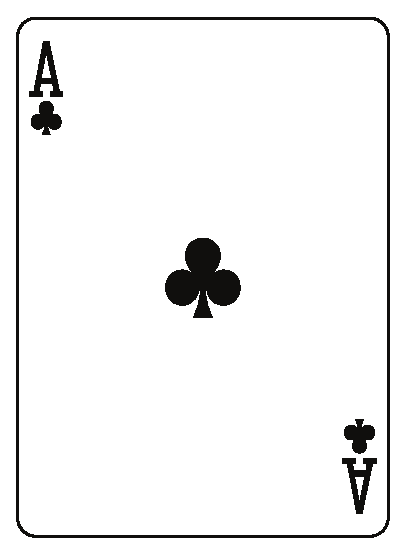
\includegraphics[width=\linewidth]{im/clubs_a.eps}
   \end{figure}
  \end{column}
  
  \begin{column}{7cm}
   \begin{itemize}[label=$\clubsuit$]
    \item Drinking game
    \item Players have to avoid getting smashed
   \end{itemize}
  \end{column}

 \end{columns}

\end{frame}

\frame{\frametitle{Game explanation}
\begin{itemize}[label=$\clubsuit$]
\item Playing a round
\item Strategies
\end{itemize}
}
\frame{\frametitle{Types of logic}
\begin{itemize}[label=$\clubsuit$]
\item Epistemic logic
\item Public announcement
\end{itemize}
}

\section{Formalizing the game}
\begin{frame}
\frametitle{Kripke structure}
 \begin{columns}
  \begin{column}{3cm}
   \begin{figure}
    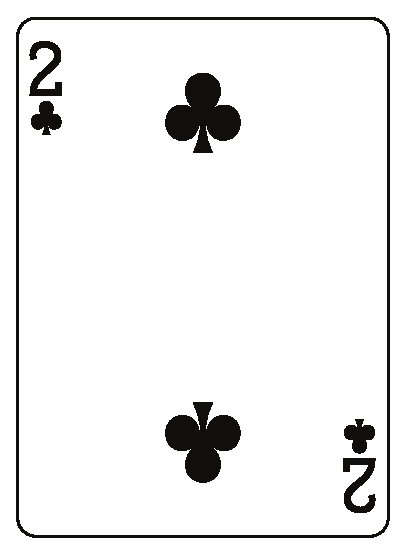
\includegraphics[width=\linewidth]{im/clubs_2.eps}
   \end{figure}
  \end{column}
  
  \begin{column}{7cm}
    \begin{itemize}[label=$\clubsuit$]
    \item $M = \langle S, \pi, R \rangle$
    \item States are given by $\boldsymbol s = (s_1,s_2,\ldots,s_m) \in S$ where $s_i \in D = \{2,3,4,5,6,7,8,9,10,j,q,k,a\}$.
    \item Relations are defined as $\boldsymbol s R_i \boldsymbol t$ such that $s_j = t_j$ for all $j\neq i$.
    \end{itemize}
  \end{column}
 \end{columns}
\end{frame}

\begin{frame}
\frametitle{Kripke structure II}
 \begin{columns}
  \begin{column}{3cm}
   \begin{figure}
    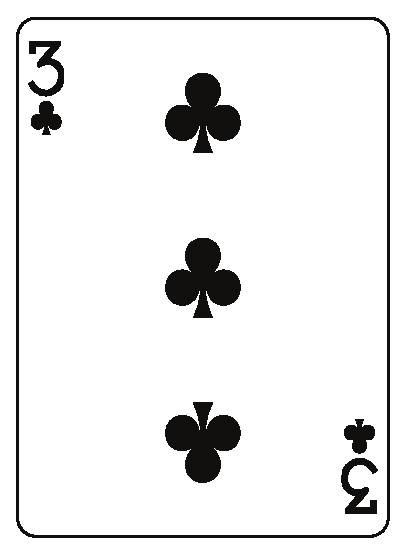
\includegraphics[width=\linewidth]{im/clubs_3.eps}
   \end{figure}
  \end{column}
  
  \begin{column}{7cm}
    \begin{itemize}[label=$\clubsuit$]
    \item Propositions $\boldsymbol P = \{ p_i c_2, p_i c_3, \ldots, p_i c_a, w_i,l_i \}^m_{i=1}$
    \item We have $\pi(\boldsymbol s)(p_i c_j) = \mathbb{t}$ iff $s_i = j$, so $\pi(\boldsymbol s)(p_ic_j) = \mathbb{f}$ iff $s_i \neq j$.
    \item Furthermore, we have $\pi(\boldsymbol s)(w_i) = \mathbb{t}$ and $\pi(\boldsymbol s)(l_i) =\mathbb{f}$ iff $s_i > s_j$ for all $j \neq i$. 
    \end{itemize}
  \end{column}
 \end{columns}
\end{frame}

\section{Analysis}
\begin{frame}
\frametitle{Combinatorial analysis}
 \begin{columns}
  \begin{column}{3cm}
   \begin{figure}
    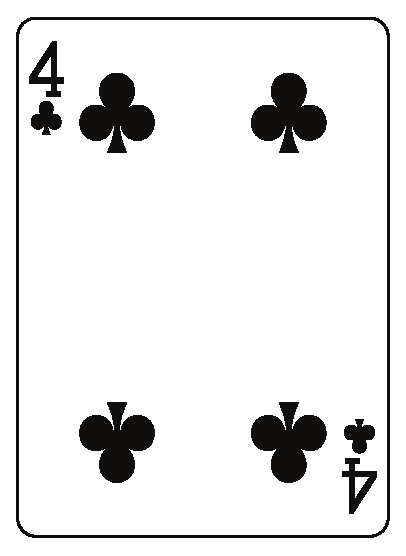
\includegraphics[width=\linewidth]{im/clubs_4.eps}
   \end{figure}
  \end{column}
  
  \begin{column}{7cm}
    \begin{itemize}[label=$\clubsuit$]
      \item Combinatorial explosion?
      \item Suppose we take a subset of the total deck $D' \subseteq D$ with $|D'| = n$. \item Let's say we have $m$ players. Before anything is known, there are $\displaystyle g=\frac{n!}{(n-m)!}$ possible games.
    \end{itemize}
    \begin{figure}
     \begin{subfigure}{.15\linewidth}
      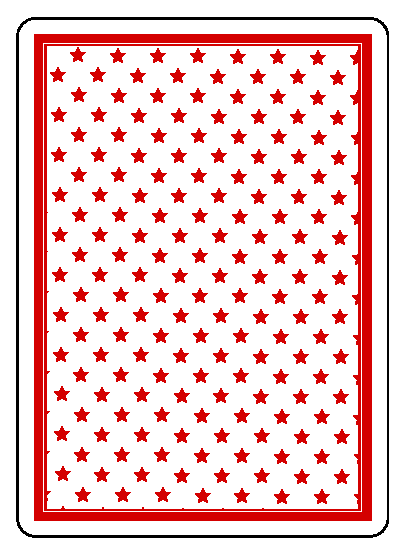
\includegraphics[width=\linewidth]{im/back.eps}
      \caption{1}
     \end{subfigure}
     \begin{subfigure}{.15\linewidth}
      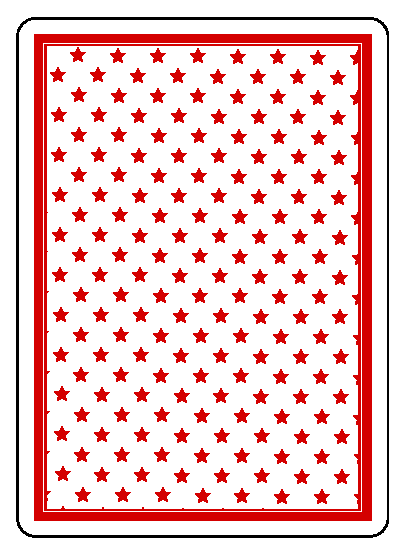
\includegraphics[width=\linewidth]{im/back.eps}
      \caption{2}
     \end{subfigure}
     \begin{subfigure}{.15\linewidth}
      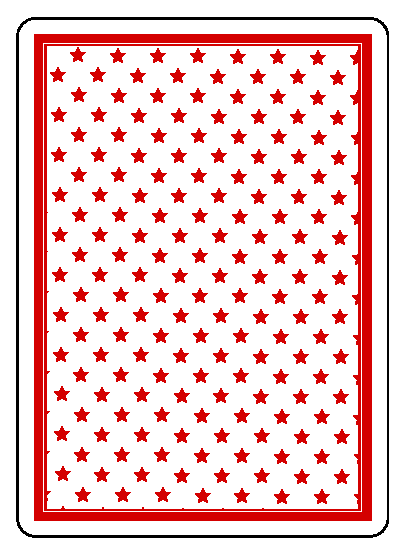
\includegraphics[width=\linewidth]{im/back.eps}
      \caption{3}
     \end{subfigure}
     \begin{subfigure}{.15\linewidth}
      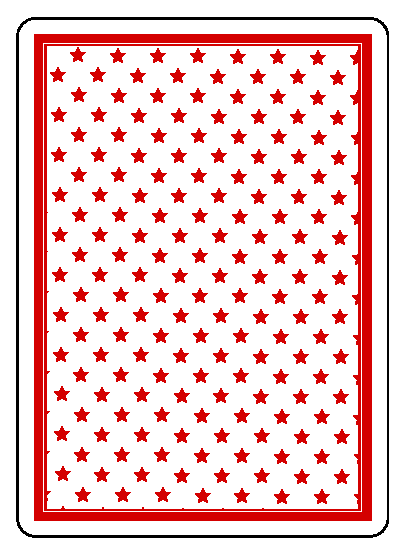
\includegraphics[width=\linewidth]{im/back.eps}
     \end{subfigure}
     \begin{subfigure}{.15\linewidth}
      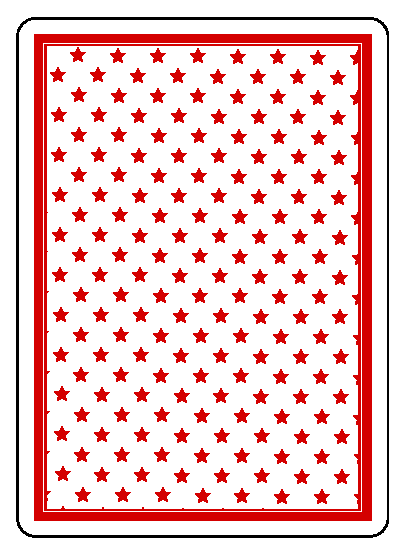
\includegraphics[width=\linewidth]{im/back.eps}
     \end{subfigure}
    \end{figure}
  \end{column}
 \end{columns}
\end{frame}

\begin{frame}
\frametitle{Combinatorial analysis II}
 \begin{columns}
  \begin{column}{3cm}
   \begin{figure}
    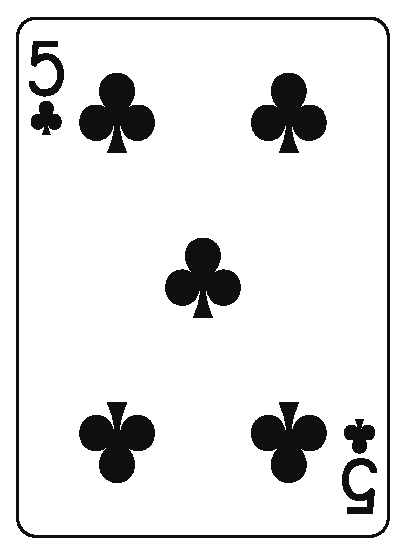
\includegraphics[width=\linewidth]{im/clubs_5.eps}
   \end{figure}
  \end{column}
  
  \begin{column}{7cm}
    \begin{itemize}[label=$\clubsuit$]
      \item Once they are drawn it isn't that bad anymore
      \item Each player has $n-m+1$ alternatives for what he is seeing
      \item Hence, there are $m(n-m+1) -m + 1$ possible worlds left
    \end{itemize}
    \begin{figure}
     \begin{subfigure}{.15\linewidth}
      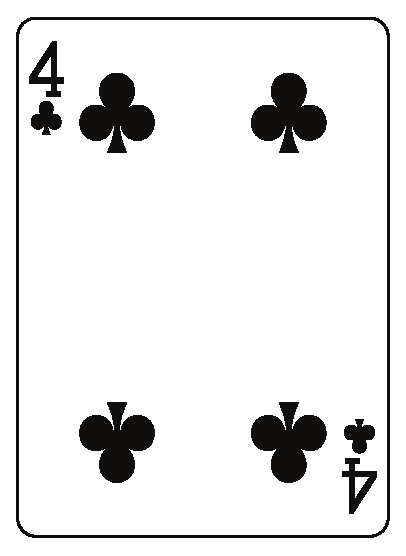
\includegraphics[width=\linewidth]{im/clubs_4.eps}
      \caption{1}
     \end{subfigure}
     \begin{subfigure}{.15\linewidth}
      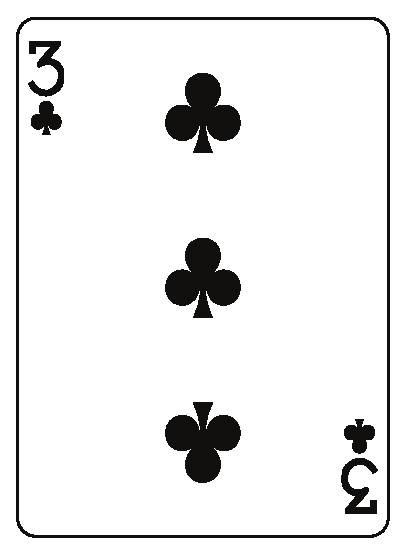
\includegraphics[width=\linewidth]{im/clubs_3.eps}
      \caption{2}
     \end{subfigure}
     \begin{subfigure}{.15\linewidth}
      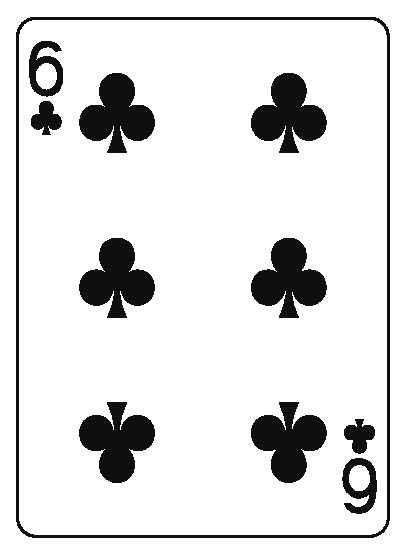
\includegraphics[width=\linewidth]{im/clubs_6.eps}
      \caption{3}
     \end{subfigure}
     \begin{subfigure}{.15\linewidth}
      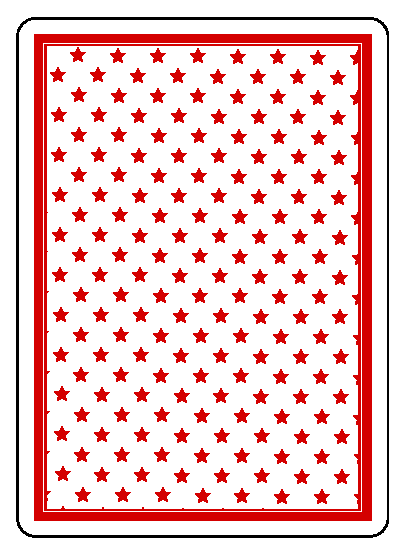
\includegraphics[width=\linewidth]{im/back.eps}
     \end{subfigure}
     \begin{subfigure}{.15\linewidth}
      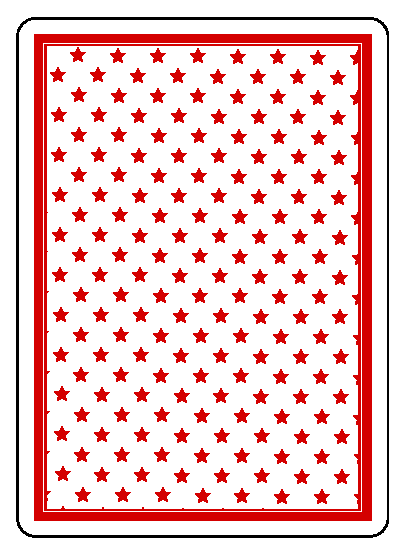
\includegraphics[width=\linewidth]{im/back.eps}
     \end{subfigure}
    \end{figure}
  \end{column}
 \end{columns}
\end{frame}


\begin{frame}
\frametitle{Game analysis}
 \begin{columns}
  \begin{column}{3cm}
   \begin{figure}
    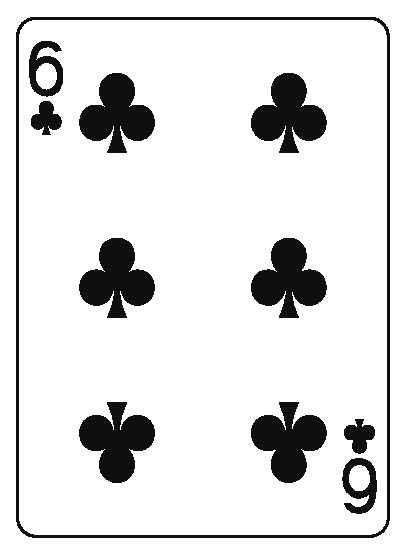
\includegraphics[width=\linewidth]{im/clubs_6.eps}
   \end{figure}
  \end{column}
  
  \begin{column}{7cm}
    \begin{itemize}[label=$\clubsuit$]
      \item First scenario: $n$ cards game with $m=n$ players.
      \item After cards are drawn only one possibility is left: 
      \begin{equation*}
	m(n-m+1) -m + 1 = 1
      \end{equation*}
    \end{itemize}
  \end{column}
 \end{columns}
\end{frame}


\begin{frame}
\frametitle{Game analysis II}
 \begin{columns}
  \begin{column}{3cm}
   \begin{figure}
    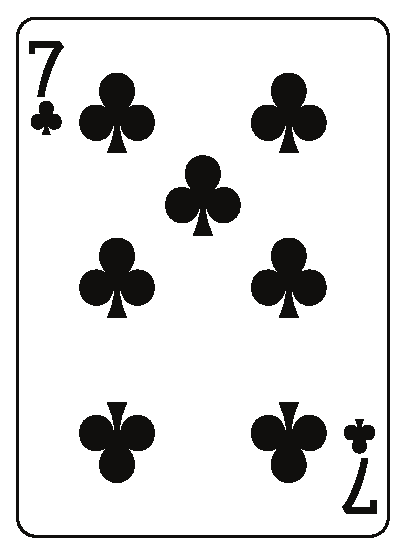
\includegraphics[width=\linewidth]{im/clubs_7.eps}
   \end{figure}
  \end{column}
  
  \begin{column}{7cm}
    \begin{itemize}[label=$\clubsuit$]
      \item Second scenario: $n$ cards with $m < n$ players
      \item Let $T_i \subseteq S$ be the subset of states such that $\boldsymbol s R_i \boldsymbol t$
      \item Estimating probability to win:
      \begin{equation*}   
\mathcal{P}^{(w_i)}_i = \frac{|T^{(w_i)}_i|}{|T_i|} = \frac{\lvert T^{(w_i)}_i\rvert}{n-m+1}
      \end{equation*}

    \end{itemize}
  \end{column}
 \end{columns}
\end{frame}


\begin{frame}
\frametitle{Strategies}
 \begin{columns}
  \begin{column}{3cm}
   \begin{figure}
    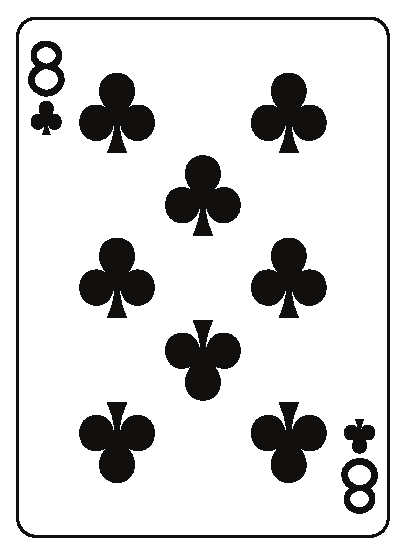
\includegraphics[width=\linewidth]{im/clubs_8.eps}
   \end{figure}
  \end{column}
  
  \begin{column}{7cm}
    \begin{itemize}[label=$\clubsuit$]
      \item Let $\mathcal G^{(k)}$ be the gain of winning the in betting round $k$. We define the utility for winning as:
     \[
	U_i^{(w_i)} = \mathcal G^{(k)}_i \mathcal P ^{(w_i)}_i
     \]
     \item And for losing:
     \[
	U^{(l_i)}_i = -\mathcal L^{k}_i (1-\mathcal P^{(w_i)}_i)
     \]
     in which $\mathcal L^{(k)}_i$ denotes the loss
    \end{itemize}
  \end{column}
 \end{columns}
\end{frame}



\begin{frame}
\frametitle{Deciding to call}
 \begin{columns}
  \begin{column}{3cm}
   \begin{figure}
    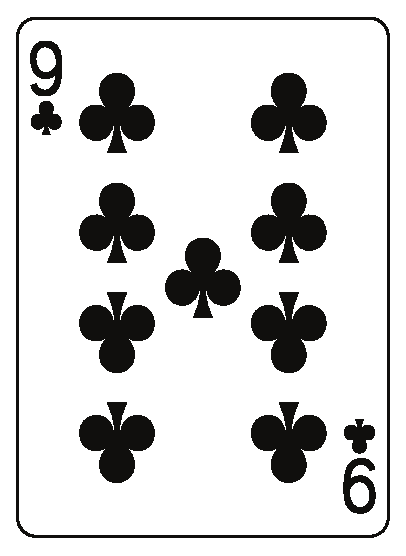
\includegraphics[width=\linewidth]{im/clubs_9.eps}
   \end{figure}
  \end{column}
  
  \begin{column}{7cm}
    \begin{itemize}[label=$\clubsuit$]
     \item Let's simplify things by saying that there is only one round for players to bet
     \item A player decides to call with 1 sip iff
     \[
	\gamma_i U_i^{(w_i)} + U^{(l_i)}_i \geq 0
     \]
     \item The $\gamma_i$ parameter determines the strategy of a player
     \item Risky: $\gamma_i > 1$, safe: $\gamma_i < 1$, optimal $\gamma_i=1$ 
    \end{itemize}
  \end{column}
 \end{columns}
\end{frame}


\begin{frame}
\frametitle{Inferring another player's strategy}
 \begin{columns}
  \begin{column}{3cm}
   \begin{figure}
    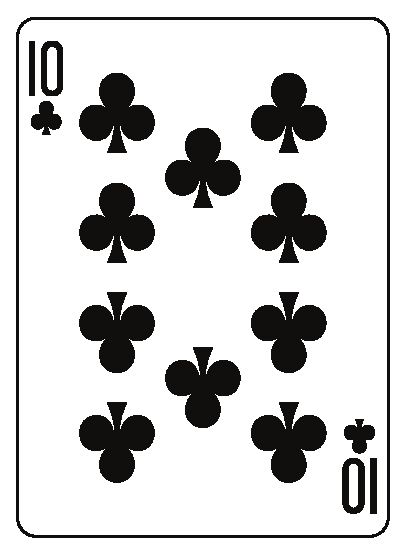
\includegraphics[width=\linewidth]{im/clubs_10.eps}
   \end{figure}
  \end{column}
  
  \begin{column}{7cm}
    \begin{itemize}[label=$\clubsuit$]
     \item We add three propositions for each player: 
     $$\boldsymbol{P}'=\boldsymbol{P} \cup \{r_i,o_i,h_i\}_{i=1}^m$$
     \item Each player knows that a player has either one of three strategies: risky $\gamma_i = 1.1$, optimal $\gamma_i = 1$ or harmless (safe) $\gamma_i = 0.9$:
    \begin{equation*}
    M \models K_i r_i \vee K_i o_i \vee K_i h_i 
    \end{equation*}
    
    \begin{align*}
    \begin{array}{ccc}
    M \models K_i \bigwedge_{j=1}^m\bigg( &(r_j \wedge \neg o_j \wedge \neg h_j ) \vee\\
					    & (\neg r_j \wedge o_j \wedge \neg h_j) \vee\\
					    & (\neg r_j \wedge \neg o_j \wedge h_j)\bigg)
    \end{array}
    \end{align*}
    \end{itemize}
  \end{column}
 \end{columns}
\end{frame}


\begin{frame}
\frametitle{Ending a round}
 \begin{columns}
  \begin{column}{3cm}
   \begin{figure}
    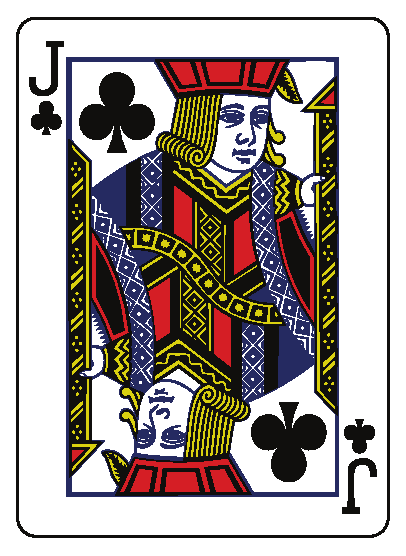
\includegraphics[width=\linewidth]{im/clubs_J.eps}
   \end{figure}
  \end{column}
  
  \begin{column}{7cm}
    \begin{itemize}[label=$\clubsuit$	]
     \item If a player called, the others can know that
     \begin{align*}
\gamma_i U^{(w_i)}_i + U^{(l_i)}_i &\geq 0\\
\gamma_i &\geq -\frac{U^{(l_i)}_i }{U^{(w_i)}_i}\\
\end{align*}
    \item Similarly, when a player folded:
    \begin{align*}
\gamma_i U^{(w_i)}_i + U^{(l_i)}_i &< 0\\
\gamma_i &< -\frac{U^{(l_i)}_i }{U^{(w_i)}_i}\\
\end{align*}

    \end{itemize}
  \end{column}
 \end{columns}
\end{frame}


\begin{frame}
\frametitle{Playing multiple rounds}
 \begin{columns}
  \begin{column}{3cm}
   \begin{figure}
    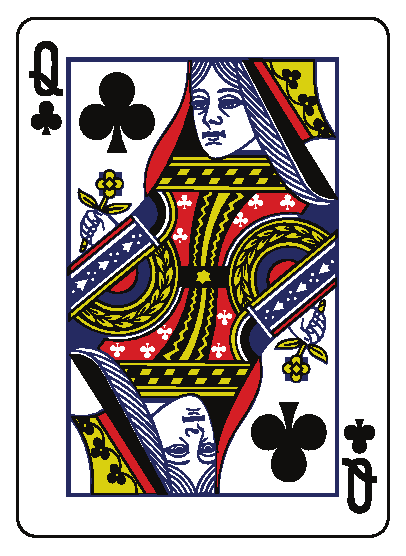
\includegraphics[width=\linewidth]{im/clubs_Q.eps}
   \end{figure}
  \end{column}
  
  \begin{column}{7cm}
    \begin{itemize}[label=$\clubsuit$]
     \item We can consider these events as announcements about $r_i$, $o_i$ and $h_i$
     \item Suppose we have played three rounds in which $\gamma_i < 1.5$, $\gamma_i \geq 0.93$ and $\gamma_i < 1.06$.
     \begin{equation*}
      M\models [r_i \vee o_i \vee h_i][\neg h_i][\neg r_i] \bigwedge_{j=1}^m K_j o_i
    \end{equation*}
    \end{itemize}
  \end{column}
 \end{columns}
\end{frame}


\frame{\frametitle{Game simulation}
\textbf{Simulation of the game}\\
\url{http://jostosh.github.io/website/index.html}
}
\frame{\frametitle{Playing the game}
\begin{itemize}[label=$\clubsuit$]
\item
\item
\end{itemize}
}
\frame{\frametitle{Conclusion}

}
\plain{Questions?}
\end{document}
